\documentclass[11pt,a4paper]{article}

% ── Packages ──────────────────────────────────────────────────────────
\usepackage[utf8]{inputenc}
\usepackage[T1]{fontenc}
\usepackage{lmodern}
\usepackage[margin=1in]{geometry}
\usepackage{graphicx}
\usepackage{amsmath,amssymb}
\usepackage{enumitem}
\usepackage{hyperref}
\usepackage{xcolor}
\usepackage{listings}
\usepackage{tikz}
\usetikzlibrary{shapes,arrows.meta,positioning,fit,calc}
\usepackage{booktabs}
\usepackage{multicol}
\usepackage{fancyhdr}
\usepackage{tcolorbox}
\tcbuselibrary{listings,skins,breakable}
\usepackage{titlesec}

% ── Styling ───────────────────────────────────────────────────────────
\hypersetup{colorlinks=true,linkcolor=blue!60!black,urlcolor=blue!70!black}

\definecolor{codebg}{RGB}{245,245,245}
\definecolor{codeframe}{RGB}{200,200,200}
\definecolor{keywordcol}{RGB}{0,0,180}
\definecolor{stringcol}{RGB}{163,21,21}
\definecolor{commentcol}{RGB}{0,128,0}
\definecolor{sectionblue}{RGB}{0,51,102}
\definecolor{tipgreen}{RGB}{34,139,34}
\definecolor{warnred}{RGB}{178,34,34}

\lstset{
  basicstyle=\ttfamily\small,
  backgroundcolor=\color{codebg},
  frame=single,
  rulecolor=\color{codeframe},
  keywordstyle=\color{keywordcol}\bfseries,
  stringstyle=\color{stringcol},
  commentstyle=\color{commentcol}\itshape,
  breaklines=true,
  breakatwhitespace=true,
  showstringspaces=false,
  tabsize=2,
  numbers=left,
  numberstyle=\tiny\color{gray},
  numbersep=8pt,
  xleftmargin=15pt,
  framexleftmargin=15pt,
}

\newtcolorbox{keybox}[1][]{
  colback=blue!5!white,
  colframe=sectionblue,
  fonttitle=\bfseries,
  title={#1},
  breakable
}

\newtcolorbox{tipbox}[1][]{
  colback=green!5!white,
  colframe=tipgreen,
  fonttitle=\bfseries,
  title={#1},
  breakable
}

\newtcolorbox{warnbox}[1][]{
  colback=red!5!white,
  colframe=warnred,
  fonttitle=\bfseries,
  title={#1},
  breakable
}

\titleformat{\section}{\Large\bfseries\color{sectionblue}}{\thesection}{1em}{}
\titleformat{\subsection}{\large\bfseries\color{sectionblue!80}}{\thesubsection}{1em}{}
\titleformat{\subsubsection}{\normalsize\bfseries\color{sectionblue!60}}{\thesubsubsection}{1em}{}

\pagestyle{fancy}
\fancyhf{}
\fancyhead[L]{\small\textcolor{gray}{Micron AI Agent Interview Preparation}}
\fancyhead[R]{\small\textcolor{gray}{Khushal Bhalia}}
\fancyfoot[C]{\thepage}

% ── Document ──────────────────────────────────────────────────────────
\begin{document}

% ── Title Page ────────────────────────────────────────────────────────
\begin{titlepage}
\centering
\vspace*{2cm}
{\Huge\bfseries\color{sectionblue} Micron AI Agentic Solutions\\[0.3cm]
Interview Preparation Guide}\\[1.5cm]
{\Large Khushal Bhalia}\\[0.5cm]
{\large Comprehensive Study Material}\\[2cm]
{\large\today}\\[3cm]
\textit{Covering: Transformers, LLMs, AI Agents, RAG, Multi-Agent Systems,\\
Agentic Frameworks, Vector Databases, and Project Deep-Dives}
\vfill
\end{titlepage}

\tableofcontents
\newpage

% ======================================================================
%  PART I: FOUNDATIONS
% ======================================================================
\section{Word2Vec and Word Embeddings}

\subsection{What Is Word2Vec?}
Word2Vec (Mikolov et al., 2013, Google) learns dense vector representations of words from large corpora.
Unlike one-hot encoding, these vectors capture \textbf{semantic relationships}:
$\vec{\text{king}} - \vec{\text{man}} + \vec{\text{woman}} \approx \vec{\text{queen}}$.

\subsection{Two Architectures}

\begin{keybox}[CBOW (Continuous Bag of Words)]
\begin{itemize}[nosep]
  \item \textbf{Input:} Context words (surrounding words).
  \item \textbf{Output:} Predict the center/target word.
  \item Faster to train; works well on frequent words.
  \item Example: ``The cat \underline{sat} on the mat'' --- given \{The, cat, on, the\}, predict ``sat''.
\end{itemize}
\end{keybox}

\begin{keybox}[Skip-gram]
\begin{itemize}[nosep]
  \item \textbf{Input:} The center/target word.
  \item \textbf{Output:} Predict the context words.
  \item Slower but better for rare words and small corpora.
  \item Example: Given ``sat'', predict \{The, cat, on, the, mat\}.
\end{itemize}
\end{keybox}

\subsection{Training Details}
\begin{itemize}[nosep]
  \item \textbf{Window Size:} How many surrounding words to consider (typically 2--10).
  \item \textbf{Negative Sampling:} Instead of updating all weights, sample a few ``negative'' (random) words. This makes training tractable for large vocabularies.
  \item \textbf{Hierarchical Softmax:} Uses a binary tree to reduce softmax computation from $O(V)$ to $O(\log V)$.
  \item Typical dimensionality: 100--300.
\end{itemize}

\subsection{Limitations of Word2Vec}
\begin{itemize}[nosep]
  \item \textbf{Static embeddings}: One vector per word regardless of context (``bank'' in ``river bank'' vs.\ ``bank account'' get the same vector).
  \item No sub-word information (misspellings and morphology are not handled).
  \item Solved by: \textbf{FastText} (sub-word n-grams), \textbf{ELMo} (contextual from BiLSTM), \textbf{BERT} (contextual from Transformers).
\end{itemize}

\begin{tipbox}[Interview Tip]
Be ready to explain the difference between static embeddings (Word2Vec, GloVe) and contextual embeddings (ELMo, BERT). Also know: GloVe uses matrix factorization on co-occurrence matrix; Word2Vec uses a shallow neural network.
\end{tipbox}

% ======================================================================
\section{Tokenization and Embeddings}

\subsection{Why Tokenization Matters}
Models cannot process raw text; they need numerical tokens. The tokenizer converts text $\rightarrow$ token IDs $\rightarrow$ embeddings.

\subsection{Tokenization Methods}

\begin{keybox}[Tokenization Approaches]
\begin{enumerate}[nosep]
  \item \textbf{Word-level:} Split by whitespace/punctuation. Simple but huge vocabulary; OOV (out-of-vocabulary) problem.
  \item \textbf{Character-level:} Each character is a token. Small vocab but very long sequences; loses word-level semantics.
  \item \textbf{Sub-word (BPE -- Byte Pair Encoding):} Used by GPT. Start with character vocabulary; iteratively merge the most frequent adjacent pairs. Balances vocabulary size and sequence length.
  \item \textbf{WordPiece:} Used by BERT. Similar to BPE but merges based on likelihood increase rather than frequency.
  \item \textbf{Unigram / SentencePiece:} Used by T5, LLaMA. Starts with a large vocabulary and iteratively prunes tokens that contribute least to likelihood.
\end{enumerate}
\end{keybox}

\subsection{Embeddings in Transformers}
In a Transformer, each token ID maps to a learned embedding vector via a lookup table (embedding matrix $E \in \mathbb{R}^{V \times d}$):
\[
  \text{token\_id} \xrightarrow{\text{lookup}} \mathbf{e}_i \in \mathbb{R}^d
\]
Additionally, \textbf{positional encodings} are added so the model knows token order:
\[
  \mathbf{x}_i = \mathbf{e}_i + \mathbf{p}_i
\]

\textbf{Sinusoidal Positional Encoding} (original Transformer):
\begin{align}
PE_{(pos, 2i)}   &= \sin\!\left(\frac{pos}{10000^{2i/d}}\right) \\
PE_{(pos, 2i+1)} &= \cos\!\left(\frac{pos}{10000^{2i/d}}\right)
\end{align}

Modern models (GPT, LLaMA) use \textbf{Rotary Position Embeddings (RoPE)} which encode relative positions via rotation matrices applied in the attention computation.

% ======================================================================
\section{Transformer Architecture (In Depth)}

\subsection{High-Level Overview}
The Transformer (Vaswani et al., 2017 --- ``Attention Is All You Need'') replaced recurrence with \textbf{self-attention}, enabling parallelism and capturing long-range dependencies.

\begin{center}
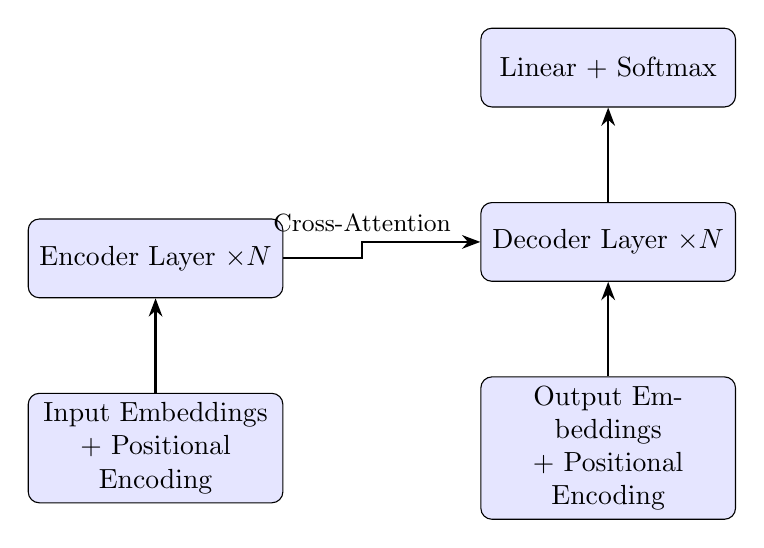
\begin{tikzpicture}[
  block/.style={rectangle, draw, fill=blue!10, text width=3cm, minimum height=1cm, align=center, rounded corners},
  arrow/.style={-Stealth, thick},
  node distance=1.2cm
]
  \node[block] (input) {Input Embeddings\\+ Positional Encoding};
  \node[block, above=of input] (enc1) {Encoder Layer $\times N$};
  \node[block, right=2.5cm of input] (output) {Output Embeddings\\+ Positional Encoding};
  \node[block, above=of output] (dec1) {Decoder Layer $\times N$};
  \node[block, above=of dec1] (linear) {Linear + Softmax};

  \draw[arrow] (input) -- (enc1);
  \draw[arrow] (output) -- (dec1);
  \draw[arrow] (enc1.east) -- ++(1,0) |- (dec1.west) node[midway, above, font=\small]{Cross-Attention};
  \draw[arrow] (dec1) -- (linear);
\end{tikzpicture}
\end{center}

\subsection{Encoder Block (Detailed)}
Each encoder layer consists of:
\begin{enumerate}[nosep]
  \item \textbf{Multi-Head Self-Attention (MHSA)}
  \item \textbf{Add \& Norm} (Residual connection + Layer Normalization)
  \item \textbf{Feed-Forward Network (FFN)} --- two linear layers with ReLU/GELU
  \item \textbf{Add \& Norm}
\end{enumerate}

\subsection{Decoder Block (Detailed)}
Each decoder layer has:
\begin{enumerate}[nosep]
  \item \textbf{Masked Multi-Head Self-Attention} (prevents attending to future tokens)
  \item Add \& Norm
  \item \textbf{Multi-Head Cross-Attention} (attends to encoder output)
  \item Add \& Norm
  \item Feed-Forward Network
  \item Add \& Norm
\end{enumerate}

\subsection{Self-Attention Mechanism (Core of Transformers)}

\begin{keybox}[Scaled Dot-Product Attention]
Given an input sequence $X \in \mathbb{R}^{n \times d}$:

\textbf{Step 1: Project into Q, K, V}
\[
Q = X W^Q, \quad K = X W^K, \quad V = X W^V
\]
where $W^Q, W^K \in \mathbb{R}^{d \times d_k}$ and $W^V \in \mathbb{R}^{d \times d_v}$.

\textbf{Step 2: Compute Attention Scores}
\[
\text{score}(Q,K) = \frac{Q K^\top}{\sqrt{d_k}}
\]
The $\sqrt{d_k}$ scaling prevents dot products from growing too large (which would push softmax into saturation regions with vanishing gradients).

\textbf{Step 3: Apply Softmax}
\[
\alpha = \text{softmax}\!\left(\frac{Q K^\top}{\sqrt{d_k}}\right)
\]
Each row of $\alpha$ is an attention distribution over all positions.

\textbf{Step 4: Weighted Sum of Values}
\[
\text{Attention}(Q,K,V) = \alpha \cdot V = \text{softmax}\!\left(\frac{Q K^\top}{\sqrt{d_k}}\right) V
\]
\end{keybox}

\subsubsection{Why Q, K, V?}
\begin{itemize}[nosep]
  \item \textbf{Query (Q):} ``What am I looking for?'' --- represents the current token's information need.
  \item \textbf{Key (K):} ``What do I contain?'' --- represents what each token offers.
  \item \textbf{Value (V):} ``What information do I actually provide?'' --- the content to aggregate.
  \item Analogy: Like a database lookup --- Query matches against Keys to find relevant Values.
\end{itemize}

\subsection{Multi-Head Attention}
Instead of one attention function, use $h$ parallel heads:
\[
\text{MultiHead}(Q,K,V) = \text{Concat}(\text{head}_1, \ldots, \text{head}_h) W^O
\]
where $\text{head}_i = \text{Attention}(Q W_i^Q, K W_i^K, V W_i^V)$.

\textbf{Why multiple heads?}
Each head can learn different types of relationships:
\begin{itemize}[nosep]
  \item Head 1 might learn syntactic dependencies (subject-verb).
  \item Head 2 might learn coreference (pronoun to noun).
  \item Head 3 might learn positional patterns.
\end{itemize}

Typical: $d_{\text{model}} = 512$, $h = 8$ heads, so $d_k = d_v = 512/8 = 64$.

\subsection{Feed-Forward Network (FFN)}
\[
\text{FFN}(x) = \text{GELU}(x W_1 + b_1) W_2 + b_2
\]
Usually $d_{\text{ff}} = 4 \times d_{\text{model}}$ (e.g., 2048 for $d_{\text{model}}=512$).

The FFN processes each position independently --- it is where the model stores ``knowledge'' (factual information from training).

\subsection{Residual Connections and Layer Normalization}
\[
\text{output} = \text{LayerNorm}(x + \text{SubLayer}(x))
\]
\begin{itemize}[nosep]
  \item \textbf{Residual connections:} Allow gradients to flow directly; prevent vanishing gradients in deep networks.
  \item \textbf{Layer Normalization:} Normalizes across features (not batch); stabilizes training.
  \item Modern LLMs use \textbf{Pre-Norm} (normalize before sublayer) instead of Post-Norm for more stable training.
  \item Many use \textbf{RMSNorm} (simpler, no mean subtraction) instead of LayerNorm.
\end{itemize}

\subsection{Masked Self-Attention in Decoders}
In autoregressive generation, the model must not see future tokens:
\[
\text{mask}_{ij} = \begin{cases} 0 & \text{if } j \leq i \\ -\infty & \text{if } j > i \end{cases}
\]
Applied before softmax: $\text{softmax}\!\left(\frac{QK^\top}{\sqrt{d_k}} + \text{mask}\right)$.

\subsection{Encoder-Decoder vs.\ Decoder-Only vs.\ Encoder-Only}

\begin{center}
\begin{tabular}{lccc}
\toprule
\textbf{Architecture} & \textbf{Example Models} & \textbf{Best For} & \textbf{Attention Type} \\
\midrule
Encoder-only & BERT, RoBERTa & Classification, NER & Bidirectional \\
Decoder-only & GPT, LLaMA, Mistral & Text generation & Causal (left-to-right) \\
Encoder-Decoder & T5, BART, mBART & Translation, Summarization & Full + Causal \\
\bottomrule
\end{tabular}
\end{center}

\begin{tipbox}[Interview Tip --- Attention Deep Dive]
Be prepared to:
\begin{itemize}[nosep]
  \item Write the attention formula from scratch.
  \item Explain why we scale by $\sqrt{d_k}$.
  \item Explain the difference between self-attention and cross-attention.
  \item Explain the masking mechanism in decoders.
  \item Discuss attention complexity $O(n^2 d)$ and efficient alternatives (Flash Attention, Sparse Attention, Sliding Window Attention used in Mistral).
\end{itemize}
\end{tipbox}

% ======================================================================
\section{LLMs vs.\ SLMs (Large vs.\ Small Language Models)}

\subsection{Definitions}
\begin{itemize}[nosep]
  \item \textbf{LLM (Large Language Model):} 7B+ parameters. Examples: GPT-4 ($\sim$1.8T), LLaMA-3 70B, Claude 3.5.
  \item \textbf{SLM (Small Language Model):} < 7B parameters. Examples: Phi-3 (3.8B), Gemma 2B, Mistral 7B, TinyLlama 1.1B.
\end{itemize}

\subsection{Comparison}

\begin{center}
\begin{tabular}{lcc}
\toprule
\textbf{Aspect} & \textbf{LLMs} & \textbf{SLMs} \\
\midrule
Parameters & 7B -- 1.8T & 1B -- 7B \\
Training Data & Trillions of tokens & Curated, smaller datasets \\
Inference Cost & High (needs GPUs) & Low (can run on edge) \\
Latency & Higher & Lower \\
Accuracy (general) & Higher & Task-dependent \\
Fine-tuning Cost & Expensive & Affordable \\
Deployment & Cloud/API & On-device, edge, local \\
Use Case & General-purpose & Domain-specific, embedded \\
\bottomrule
\end{tabular}
\end{center}

\subsection{When to Use Which}
\begin{itemize}[nosep]
  \item \textbf{Use LLMs:} Complex reasoning, multi-step tasks, code generation, general assistants.
  \item \textbf{Use SLMs:} Edge deployment (phones, IoT), low-latency needs, privacy-sensitive (on-prem), cost-sensitive applications, domain-specific fine-tuned tasks.
  \item \textbf{Micron relevance:} As a memory company, Micron is interested in running AI models efficiently on-device, making SLMs very relevant.
\end{itemize}

% ======================================================================
\section{Training Paradigms}

\subsection{Pre-training}
\begin{itemize}[nosep]
  \item Train on massive unlabeled corpora (internet text).
  \item \textbf{Causal Language Modeling (CLM):} Predict next token. Used by GPT family.
  \item \textbf{Masked Language Modeling (MLM):} Mask 15\% of tokens, predict them. Used by BERT.
  \item \textbf{Span Corruption:} Mask spans of tokens, generate them. Used by T5.
  \item Cost: Millions of dollars, weeks on thousands of GPUs.
\end{itemize}

\subsection{Fine-tuning}
\begin{itemize}[nosep]
  \item Adapt a pre-trained model to a specific task or domain.
  \item \textbf{Full fine-tuning:} Update all parameters. Best results but expensive.
  \item \textbf{Parameter-Efficient Fine-Tuning (PEFT):}
    \begin{itemize}[nosep]
      \item \textbf{LoRA (Low-Rank Adaptation):} Add low-rank matrices $\Delta W = BA$ where $B \in \mathbb{R}^{d \times r}$, $A \in \mathbb{R}^{r \times d}$, $r \ll d$. Only train $A$ and $B$.
      \item \textbf{QLoRA:} LoRA + 4-bit quantized base model. Enables fine-tuning 65B models on a single 48GB GPU.
      \item \textbf{Adapters:} Small bottleneck layers inserted into Transformer blocks.
      \item \textbf{Prefix Tuning:} Learn ``virtual prefix'' tokens prepended to keys/values.
    \end{itemize}
\end{itemize}

\subsection{Alignment: RLHF and DPO}
\begin{itemize}[nosep]
  \item \textbf{Supervised Fine-Tuning (SFT):} Train on human-written instruction-response pairs.
  \item \textbf{RLHF (Reinforcement Learning from Human Feedback):}
    \begin{enumerate}[nosep]
      \item Train a reward model on human preference data (response A vs.\ B).
      \item Optimize the LLM using PPO (Proximal Policy Optimization) to maximize the reward.
    \end{enumerate}
  \item \textbf{DPO (Direct Preference Optimization):} Skip the reward model; directly optimize the LLM on preference pairs using a classification-like loss. Simpler and increasingly popular.
\end{itemize}

\subsection{Inference-Time Optimization}
\begin{itemize}[nosep]
  \item \textbf{Quantization:} Reduce precision (FP32 $\to$ INT8/INT4). GPTQ, AWQ, GGUF formats.
  \item \textbf{KV-Cache:} Cache key/value matrices across generation steps to avoid recomputation.
  \item \textbf{Speculative Decoding:} Use a small draft model to generate candidate tokens; large model verifies in parallel.
  \item \textbf{Flash Attention:} Tiling-based attention that reduces memory from $O(n^2)$ to $O(n)$ by avoiding materializing the full attention matrix.
\end{itemize}

% ======================================================================
\section{Scaling Laws}

\subsection{Kaplan / Chinchilla Scaling Laws}

\begin{keybox}[Chinchilla Scaling Law (Hoffmann et al., 2022)]
For compute-optimal training:
\[
  D \approx 20 \times N
\]
where $N$ = number of parameters, $D$ = number of training tokens.

A 10B parameter model should be trained on $\sim$200B tokens.

The original GPT-3 (175B params, 300B tokens) was \textbf{undertrained} by this law. Chinchilla (70B params, 1.4T tokens) matched GPT-3 performance with less compute.
\end{keybox}

\subsection{Key Insights}
\begin{itemize}[nosep]
  \item Loss follows a \textbf{power law} with compute, data, and model size:
  \[
    L(N, D) \propto N^{-\alpha} + D^{-\beta} + \text{irreducible loss}
  \]
  \item There are diminishing returns; doubling parameters doesn't halve the loss.
  \item \textbf{Emergent abilities}: Some capabilities (chain-of-thought, in-context learning) appear only above certain model sizes.
  \item Modern trend: Over-train smaller models (LLaMA-3 8B trained on 15T tokens, far exceeding Chinchilla optimal) for better inference efficiency.
\end{itemize}

% ======================================================================
\section{Multilingualism and Multimodality}

\subsection{Multilingual Models}
\begin{itemize}[nosep]
  \item \textbf{mBERT, XLM-R:} Encoder models trained on 100+ languages.
  \item \textbf{mBART, mT5:} Encoder-decoder for multilingual generation/translation.
  \item \textbf{Cross-lingual transfer:} Train on English, evaluate on Hindi --- works because of shared sub-word tokens and aligned representations.
  \item \textbf{Challenges:} Curse of multilinguality (capacity dilution), low-resource languages underrepresented, tokenizer bias (non-Latin scripts get more tokens per word).
\end{itemize}

\subsection{Multimodal Models}
\begin{itemize}[nosep]
  \item \textbf{Vision-Language:} GPT-4V, LLaVA, Gemini --- process both images and text.
  \item \textbf{Architecture:} Vision encoder (ViT/CLIP) produces image tokens; these are projected into the LLM's embedding space and concatenated with text tokens.
  \item \textbf{CLIP (Contrastive Language--Image Pre-training):} Learns aligned image-text embeddings via contrastive loss. Used for zero-shot image classification and retrieval.
  \item \textbf{Audio:} Whisper (speech-to-text), AudioLM.
  \item \textbf{Video:} Typically frame sampling + vision encoder per frame.
\end{itemize}

% ======================================================================
\section{Mixture of Experts (MoE)}

\subsection{Concept}
Instead of one large FFN, have $E$ expert FFNs but only activate $k$ per token (sparse activation):
\[
  y = \sum_{i=1}^{E} g_i(x) \cdot \text{Expert}_i(x), \quad \text{where only top-}k\ g_i \neq 0
\]

\subsection{Router/Gating Network}
\[
  g(x) = \text{TopK}\!\left(\text{softmax}(W_g \cdot x)\right)
\]
The router decides which experts to activate for each token.

\subsection{Examples and Key Points}
\begin{itemize}[nosep]
  \item \textbf{Mixtral 8x7B:} 8 experts, top-2 routing. Total params: 46.7B, active per token: $\sim$12.9B. Performance comparable to LLaMA-2 70B.
  \item \textbf{GPT-4:} Rumored to use MoE with 8 experts of $\sim$220B each.
  \item \textbf{Benefits:} More parameters (knowledge capacity) without proportional compute increase.
  \item \textbf{Challenges:} Load balancing (some experts get all tokens), training instability, higher memory (all experts must be in memory even if not all are active).
  \item \textbf{Auxiliary loss:} Added during training to encourage balanced expert utilization.
\end{itemize}

% ======================================================================
\section{Vector Databases}

\subsection{What Are They?}
Databases optimized for storing, indexing, and querying high-dimensional vectors (embeddings). Essential for similarity search in AI applications.

\subsection{Key Concepts}
\begin{itemize}[nosep]
  \item \textbf{Embedding:} Dense vector representation of text/image/audio (e.g., 768-d or 1536-d).
  \item \textbf{Similarity Metrics:}
    \begin{itemize}[nosep]
      \item \textbf{Cosine Similarity:} $\cos(\mathbf{a}, \mathbf{b}) = \frac{\mathbf{a} \cdot \mathbf{b}}{\|\mathbf{a}\| \|\mathbf{b}\|}$ --- measures angle; ignores magnitude.
      \item \textbf{Euclidean Distance (L2):} $\|\mathbf{a} - \mathbf{b}\|_2$ --- measures absolute distance.
      \item \textbf{Dot Product:} $\mathbf{a} \cdot \mathbf{b}$ --- used when magnitude matters.
    \end{itemize}
  \item \textbf{Approximate Nearest Neighbor (ANN):} Exact search is $O(n)$; ANN algorithms trade accuracy for speed.
\end{itemize}

\subsection{Indexing Algorithms}
\begin{itemize}[nosep]
  \item \textbf{HNSW (Hierarchical Navigable Small World):} Graph-based. Fast queries, high recall. Used by most vector DBs.
  \item \textbf{IVF (Inverted File Index):} Cluster vectors; search only relevant clusters.
  \item \textbf{PQ (Product Quantization):} Compress vectors for memory efficiency.
  \item \textbf{FAISS:} Facebook's library combining IVF + PQ + HNSW.
\end{itemize}

\subsection{Popular Vector Databases}
\begin{center}
\begin{tabular}{lll}
\toprule
\textbf{Database} & \textbf{Type} & \textbf{Key Feature} \\
\midrule
Pinecone & Managed cloud & Serverless, easy to use \\
Weaviate & Open-source & Hybrid search (vector + keyword) \\
Chroma & Open-source & Lightweight, good for prototyping \\
Qdrant & Open-source & Rust-based, fast \\
Milvus & Open-source & Scalable, enterprise-grade \\
pgvector & Extension & PostgreSQL extension for vectors \\
\bottomrule
\end{tabular}
\end{center}

% ======================================================================
\section{RAG (Retrieval-Augmented Generation)}

\subsection{The Problem RAG Solves}
LLMs have a knowledge cutoff and can hallucinate. RAG grounds generation in retrieved documents.

\subsection{RAG Pipeline}

\begin{center}
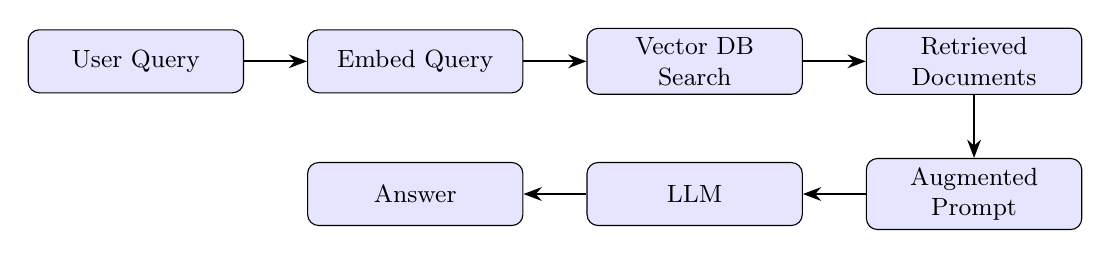
\begin{tikzpicture}[
  block/.style={rectangle, draw, fill=blue!10, text width=2.5cm, minimum height=0.8cm, align=center, rounded corners, font=\small},
  arrow/.style={-Stealth, thick},
  node distance=0.8cm
]
  \node[block] (query) {User Query};
  \node[block, right=of query] (embed) {Embed Query};
  \node[block, right=of embed] (search) {Vector DB\\Search};
  \node[block, right=of search] (context) {Retrieved\\Documents};
  \node[block, below=of context] (prompt) {Augmented\\Prompt};
  \node[block, left=of prompt] (llm) {LLM};
  \node[block, left=of llm] (answer) {Answer};

  \draw[arrow] (query) -- (embed);
  \draw[arrow] (embed) -- (search);
  \draw[arrow] (search) -- (context);
  \draw[arrow] (context) -- (prompt);
  \draw[arrow] (prompt) -- (llm);
  \draw[arrow] (llm) -- (answer);
\end{tikzpicture}
\end{center}

\subsection{Key Components}
\begin{enumerate}[nosep]
  \item \textbf{Document Ingestion:} Load documents $\rightarrow$ chunk them $\rightarrow$ embed chunks $\rightarrow$ store in vector DB.
  \item \textbf{Chunking Strategies:}
    \begin{itemize}[nosep]
      \item Fixed-size chunks (e.g., 512 tokens) with overlap (e.g., 50 tokens).
      \item Recursive character splitting (LangChain default).
      \item Semantic chunking (split at topic boundaries).
    \end{itemize}
  \item \textbf{Retrieval:} Embed query $\rightarrow$ find top-$k$ similar chunks.
  \item \textbf{Generation:} Concatenate retrieved chunks with query $\rightarrow$ send to LLM.
\end{enumerate}

\subsection{Advanced RAG Techniques}
\begin{itemize}[nosep]
  \item \textbf{Hybrid Search:} Combine vector similarity with BM25 keyword search.
  \item \textbf{Re-ranking:} Use a cross-encoder to re-rank retrieved chunks for relevance.
  \item \textbf{Query Transformation:} Rephrase or decompose complex queries.
  \item \textbf{HyDE (Hypothetical Document Embeddings):} Generate a hypothetical answer, embed it, and use that for retrieval.
  \item \textbf{Multi-query RAG:} Generate multiple query variants and retrieve for each.
  \item \textbf{Agentic RAG:} An agent decides when/what to retrieve, can do multi-step retrieval.
\end{itemize}

% ======================================================================
\section{Indexing and Searching (General)}

\subsection{Traditional Indexing}
\begin{itemize}[nosep]
  \item \textbf{Inverted Index:} Maps terms $\rightarrow$ document IDs. Core of Elasticsearch, Lucene.
  \item \textbf{B-Tree / B+ Tree:} Used in databases (PostgreSQL) for ordered data.
  \item \textbf{Hash Index:} $O(1)$ lookup; not suitable for range queries.
\end{itemize}

\subsection{Text Search}
\begin{itemize}[nosep]
  \item \textbf{TF-IDF:} Term Frequency $\times$ Inverse Document Frequency. Captures word importance.
  \[
    \text{TF-IDF}(t,d) = \text{TF}(t,d) \times \log\!\left(\frac{N}{\text{DF}(t)}\right)
  \]
  \item \textbf{BM25:} Improved TF-IDF with document length normalization. Used in Elasticsearch.
  \item \textbf{Limitations:} Cannot capture semantic similarity (``car'' vs.\ ``automobile'').
\end{itemize}

\subsection{Semantic Search}
\begin{itemize}[nosep]
  \item Embed documents and queries into the same vector space.
  \item Use ANN algorithms (HNSW, IVF) for fast retrieval.
  \item Models: Sentence-BERT, OpenAI text-embedding-ada-002, Cohere embed, BGE.
\end{itemize}

\subsection{Hybrid Search}
Combines keyword (BM25) and semantic (vector) search with score fusion:
\[
  \text{score}_{\text{final}} = \alpha \cdot \text{score}_{\text{BM25}} + (1-\alpha) \cdot \text{score}_{\text{vector}}
\]

% ======================================================================
\section{Tool Calling}

\subsection{What Is Tool Calling?}
LLMs can be given access to external \textbf{tools} (functions, APIs, databases). The model generates a structured function call (JSON) that the system executes, and the result is fed back.

\subsection{How It Works}
\begin{enumerate}[nosep]
  \item Define tools with name, description, and parameter schema (JSON Schema).
  \item Include tool definitions in the system prompt or API call.
  \item LLM decides when to call a tool and generates the function call with arguments.
  \item System executes the function and returns the result.
  \item LLM uses the result to formulate the final answer.
\end{enumerate}

\subsection{Example (OpenAI Function Calling)}
\begin{lstlisting}[language=Python]
tools = [{
    "type": "function",
    "function": {
        "name": "get_weather",
        "description": "Get current weather for a city",
        "parameters": {
            "type": "object",
            "properties": {
                "city": {"type": "string"}
            },
            "required": ["city"]
        }
    }
}]
# LLM response: {"name": "get_weather", "arguments": {"city": "Boise"}}
\end{lstlisting}

% ======================================================================
\section{A2A (Agent-to-Agent Protocol)}

\subsection{What Is A2A?}
A2A is Google's open protocol for communication between AI agents. It defines how agents discover each other's capabilities, negotiate tasks, and exchange information.

\subsection{Key Concepts}
\begin{itemize}[nosep]
  \item \textbf{Agent Card:} A JSON metadata file (at \texttt{/.well-known/agent.json}) describing an agent's capabilities, skills, and supported input/output formats.
  \item \textbf{Task:} The unit of work. Has states: \texttt{submitted} $\to$ \texttt{working} $\to$ \texttt{completed/failed}.
  \item \textbf{Message/Part:} Communication units (text, file, structured data).
  \item \textbf{Push Notifications:} Agents can subscribe to task updates via webhooks.
\end{itemize}

\subsection{A2A vs.\ MCP}
\begin{center}
\begin{tabular}{lcc}
\toprule
\textbf{Aspect} & \textbf{A2A} & \textbf{MCP} \\
\midrule
Purpose & Agent-to-agent communication & Agent-to-tool connection \\
Scope & Inter-agent collaboration & Extend single agent's capabilities \\
Analogy & Agents talking to each other & Agent using tools/APIs \\
Initiated by & Google & Anthropic \\
\bottomrule
\end{tabular}
\end{center}

% ======================================================================
\section{MCP (Model Context Protocol)}

\subsection{What Is MCP?}
MCP (by Anthropic) is an open standard for connecting LLMs to external data sources and tools. Think of it as a \textbf{USB-C port for AI} --- one protocol to connect to any tool.

\subsection{Architecture}
\begin{itemize}[nosep]
  \item \textbf{MCP Host:} The application (IDE, chatbot) that wants to access tools.
  \item \textbf{MCP Client:} Maintains a 1:1 connection with a server.
  \item \textbf{MCP Server:} Exposes capabilities (tools, resources, prompts) to the client.
\end{itemize}

\subsection{What MCP Servers Expose}
\begin{enumerate}[nosep]
  \item \textbf{Tools:} Functions the LLM can call (e.g., search database, send email).
  \item \textbf{Resources:} Data the LLM can read (e.g., files, database records).
  \item \textbf{Prompts:} Predefined prompt templates.
\end{enumerate}

\subsection{Transport Protocols}
\begin{itemize}[nosep]
  \item \textbf{stdio:} For local processes (agent and server on same machine).
  \item \textbf{HTTP + SSE (Server-Sent Events):} For remote servers.
\end{itemize}

\subsection{Why MCP Matters}
\begin{itemize}[nosep]
  \item Before MCP: Each tool integration required custom code ($N$ models $\times$ $M$ tools = $N \times M$ integrations).
  \item With MCP: Each model implements MCP client once, each tool implements MCP server once ($N + M$ integrations).
  \item Adopted by: Cursor, VS Code Copilot, Claude Desktop, Windsurf.
\end{itemize}

% ======================================================================
\section{Agentic AI Frameworks}

\subsection{LangChain}

\begin{keybox}[LangChain Core Concepts]
\begin{itemize}[nosep]
  \item \textbf{LLMs / Chat Models:} Wrappers around LLM APIs (OpenAI, Anthropic, Ollama).
  \item \textbf{Prompt Templates:} Structured prompts with variables.
  \item \textbf{Chains:} Sequential pipelines (prompt $\to$ LLM $\to$ output parser).
  \item \textbf{Agents:} LLM-powered decision makers that choose which tools to use.
  \item \textbf{Tools:} Functions agents can call (search, calculator, SQL).
  \item \textbf{Memory:} Conversation history management.
  \item \textbf{Retrievers:} Interface to vector stores for RAG.
  \item \textbf{Output Parsers:} Structure LLM output (JSON, lists).
  \item \textbf{LCEL (LangChain Expression Language):} Composable chain syntax using \texttt{|} pipe operator.
\end{itemize}
\end{keybox}

\subsection{LangGraph}
\begin{itemize}[nosep]
  \item Built on LangChain; models agent workflows as \textbf{directed graphs}.
  \item \textbf{Nodes:} Functions/agents that perform work.
  \item \textbf{Edges:} Control flow (including conditional routing).
  \item \textbf{State:} Shared state object passed between nodes.
  \item \textbf{Persistence:} Built-in checkpointing for long-running workflows.
  \item \textbf{Human-in-the-loop:} Can pause execution for human approval.
  \item Ideal for complex, multi-step agentic workflows with cycles and branching.
\end{itemize}

\subsection{CrewAI}
\begin{itemize}[nosep]
  \item Multi-agent framework with \textbf{role-based} design.
  \item \textbf{Agents:} Each has a role, goal, and backstory.
  \item \textbf{Tasks:} Assigned to specific agents with expected output.
  \item \textbf{Crew:} Orchestrates agents to complete tasks.
  \item \textbf{Process types:} Sequential, hierarchical (manager agent delegates).
  \item Simple API; good for quick multi-agent prototyping.
\end{itemize}

\subsection{AutoGen (Microsoft)}
\begin{itemize}[nosep]
  \item Framework for building multi-agent \textbf{conversations}.
  \item Agents communicate via messages (like a group chat).
  \item \textbf{AssistantAgent:} LLM-powered agent.
  \item \textbf{UserProxyAgent:} Executes code, represents human.
  \item Supports code generation, execution, and debugging in conversation.
  \item Good for collaborative problem-solving between agents.
\end{itemize}

\subsection{n8n}
\begin{itemize}[nosep]
  \item \textbf{Visual workflow automation} platform (low-code/no-code).
  \item Drag-and-drop nodes to build workflows.
  \item 400+ integrations (Slack, Gmail, databases, APIs).
  \item AI features: LLM nodes, AI agent nodes, vector store integration.
  \item Self-hostable (open-source) or cloud.
  \item Good for: Non-developers building AI-powered automations.
\end{itemize}

\subsection{Framework Comparison}
\begin{center}
\begin{tabular}{lcccc}
\toprule
\textbf{Feature} & \textbf{LangChain} & \textbf{LangGraph} & \textbf{CrewAI} & \textbf{AutoGen} \\
\midrule
Paradigm & Chains/Agents & Graph-based & Role-based & Conversation \\
Multi-agent & Basic & Advanced & Native & Native \\
State mgmt & Manual & Built-in & Automatic & Message-based \\
Complexity & Medium & High & Low & Medium \\
Best for & RAG, tools & Complex flows & Team tasks & Code tasks \\
\bottomrule
\end{tabular}
\end{center}

% ======================================================================
\section{Orchestration}

\subsection{What Is Agent Orchestration?}
The coordination layer that manages how agents execute tasks, share state, and interact.

\subsection{Orchestration Patterns}
\begin{enumerate}[nosep]
  \item \textbf{Sequential:} Agents execute one after another. Output of one feeds into the next.
  \item \textbf{Parallel:} Multiple agents execute simultaneously on independent sub-tasks.
  \item \textbf{Hierarchical:} A manager agent delegates to worker agents.
  \item \textbf{Router:} A routing agent decides which specialist agent handles a query.
  \item \textbf{Feedback Loop:} Agents iterate until quality criteria are met (reviewer + writer pattern).
\end{enumerate}

\subsection{Key Orchestration Concerns}
\begin{itemize}[nosep]
  \item \textbf{Error handling:} Retries, fallbacks, graceful degradation.
  \item \textbf{State management:} Shared state vs.\ message passing.
  \item \textbf{Token budget:} Managing context window limits across multi-step workflows.
  \item \textbf{Observability:} Logging, tracing (LangSmith, Arize Phoenix).
  \item \textbf{Guardrails:} Ensuring agents stay within bounds (safety, cost limits).
\end{itemize}

% ======================================================================
\section{Memory in AI Agents}

\subsection{Types of Memory}
\begin{enumerate}[nosep]
  \item \textbf{Short-term / Working Memory:} The current conversation context window. Limited by model's max tokens (4K--128K+).
  \item \textbf{Long-term Memory:} Persisted information across sessions.
    \begin{itemize}[nosep]
      \item \textbf{Vector store:} Embed and store past interactions; retrieve relevant ones.
      \item \textbf{Key-value store:} Store structured user preferences.
      \item \textbf{Graph memory:} Knowledge graph of entities and relationships.
    \end{itemize}
  \item \textbf{Episodic Memory:} Specific past experiences/interactions (``Last time user asked about X'').
  \item \textbf{Semantic Memory:} General knowledge/facts (``Paris is the capital of France'').
  \item \textbf{Procedural Memory:} How to do things (stored as tools/skills).
\end{enumerate}

\subsection{Memory in LangChain}
\begin{itemize}[nosep]
  \item \textbf{ConversationBufferMemory:} Store full conversation.
  \item \textbf{ConversationSummaryMemory:} Summarize older messages.
  \item \textbf{ConversationBufferWindowMemory:} Keep only last $k$ messages.
  \item \textbf{VectorStoreRetrieverMemory:} Retrieve relevant past messages via similarity search.
\end{itemize}

% ======================================================================
\section{Multi-Agent Systems}

\subsection{Why Multi-Agent?}
\begin{itemize}[nosep]
  \item Complex tasks benefit from \textbf{specialization}: each agent is an expert.
  \item Better \textbf{scalability}: add agents for new capabilities.
  \item \textbf{Modularity}: easier to develop, test, and maintain individual agents.
  \item \textbf{Robustness}: failure of one agent doesn't crash the system.
\end{itemize}

\subsection{Common Multi-Agent Patterns}
\begin{enumerate}[nosep]
  \item \textbf{Supervisor/Worker:} One supervisor delegates to specialist workers.
  \item \textbf{Debate:} Multiple agents argue for/against; synthesize best answer.
  \item \textbf{Pipeline:} Sequential processing (researcher $\to$ writer $\to$ reviewer).
  \item \textbf{Swarm:} Agents self-organize without central control (OpenAI Swarm).
  \item \textbf{Planning:} A planner agent creates a task plan; executor agents carry it out.
\end{enumerate}

\subsection{Design Considerations}
\begin{itemize}[nosep]
  \item \textbf{Communication protocol:} Shared state vs.\ message passing vs.\ A2A.
  \item \textbf{Trust and safety:} Agent actions should be sandboxed; human approval for critical actions.
  \item \textbf{Cost control:} Each agent call costs tokens; optimize for efficiency.
  \item \textbf{Evaluation:} How to measure quality of multi-agent outputs.
\end{itemize}

% ======================================================================
%  PART II: PROJECT DEEP-DIVES WITH CODE
% ======================================================================
\newpage
\section{Project 1: ClassQR --- AI-Powered Attendance System}

\subsection{System Overview}
ClassQR is a QR-code based smart attendance system that:
\begin{itemize}[nosep]
  \item Teachers generate QR codes for lectures; students scan to mark attendance in real time.
  \item Backend: Node.js + Express + PostgreSQL.
  \item AI: Natural language queries on attendance data using LangChain.
  \item Analytics: Power BI dashboards.
\end{itemize}

\subsection{Database Schema}

\begin{lstlisting}[language=SQL, caption={PostgreSQL Schema for ClassQR}]
-- Students table
CREATE TABLE students (
  student_id   SERIAL PRIMARY KEY,
  name         VARCHAR(100) NOT NULL,
  email        VARCHAR(150) UNIQUE NOT NULL,
  roll_number  VARCHAR(20) UNIQUE NOT NULL,
  department   VARCHAR(50),
  created_at   TIMESTAMP DEFAULT NOW()
);

-- Teachers table
CREATE TABLE teachers (
  teacher_id  SERIAL PRIMARY KEY,
  name        VARCHAR(100) NOT NULL,
  email       VARCHAR(150) UNIQUE NOT NULL,
  department  VARCHAR(50)
);

-- Courses table
CREATE TABLE courses (
  course_id   SERIAL PRIMARY KEY,
  course_name VARCHAR(100) NOT NULL,
  course_code VARCHAR(20) UNIQUE NOT NULL,
  teacher_id  INTEGER REFERENCES teachers(teacher_id)
);

-- Enrollments (many-to-many: students <-> courses)
CREATE TABLE enrollments (
  enrollment_id SERIAL PRIMARY KEY,
  student_id    INTEGER REFERENCES students(student_id),
  course_id     INTEGER REFERENCES courses(course_id),
  UNIQUE(student_id, course_id)
);

-- Lectures table
CREATE TABLE lectures (
  lecture_id   SERIAL PRIMARY KEY,
  course_id    INTEGER REFERENCES courses(course_id),
  lecture_date DATE NOT NULL,
  qr_token     VARCHAR(255) UNIQUE NOT NULL,
  created_at   TIMESTAMP DEFAULT NOW()
);

-- Attendance records
CREATE TABLE attendance (
  attendance_id SERIAL PRIMARY KEY,
  lecture_id    INTEGER REFERENCES lectures(lecture_id),
  student_id    INTEGER REFERENCES students(student_id),
  scanned_at    TIMESTAMP DEFAULT NOW(),
  UNIQUE(lecture_id, student_id)
);
\end{lstlisting}

\subsection{LangChain + PostgreSQL Integration (Node.js)}

This code demonstrates the core flow:
User question (chatbot) $\to$ LLM generates SQL $\to$ Query PostgreSQL $\to$ LLM interprets results $\to$ Natural language answer.

\begin{lstlisting}[language=Java, caption={ClassQR --- LangChain SQL Agent (Node.js)},
  morekeywords={const,let,async,await,import,from,export}]
// classqr-ai.js
import { ChatOpenAI } from "@langchain/openai";
import { PromptTemplate } from "@langchain/core/prompts";
import { RunnableSequence } from "@langchain/core/runnables";
import { StringOutputParser } from "@langchain/core/output_parsers";
import pg from "pg";

// --- Database connection ---
const pool = new pg.Pool({
  host: "localhost",
  port: 5432,
  database: "classqr",
  user: "postgres",
  password: "password",
});

// --- LLM setup ---
const llm = new ChatOpenAI({
  modelName: "gpt-4o-mini",
  temperature: 0,
});

// --- Schema description for the LLM ---
const DB_SCHEMA = `
Tables:
- students(student_id, name, email, roll_number, department)
- teachers(teacher_id, name, email, department)
- courses(course_id, course_name, course_code, teacher_id)
- enrollments(enrollment_id, student_id, course_id)
- lectures(lecture_id, course_id, lecture_date, qr_token)
- attendance(attendance_id, lecture_id, student_id, scanned_at)
`;

// --- Step 1: Generate SQL from natural language ---
const sqlPrompt = PromptTemplate.fromTemplate(`
You are a PostgreSQL expert. Given the database schema and a
user question, generate a valid SQL query. Return ONLY the SQL
query, nothing else.

Schema:
{schema}

Question: {question}

SQL Query:
`);

// --- Step 2: Interpret results in natural language ---
const answerPrompt = PromptTemplate.fromTemplate(`
Given the user's question and the SQL query results, provide
a clear, helpful natural language answer.

Question: {question}
SQL Query: {sql}
Results: {results}

Answer:
`);

// --- Main query function ---
async function askClassQR(question) {
  // Step 1: Generate SQL
  const sqlChain = RunnableSequence.from([
    sqlPrompt,
    llm,
    new StringOutputParser(),
  ]);

  const sqlQuery = await sqlChain.invoke({
    schema: DB_SCHEMA,
    question: question,
  });

  console.log("Generated SQL:", sqlQuery);

  // Step 2: Execute SQL against PostgreSQL
  const result = await pool.query(sqlQuery);
  const rows = JSON.stringify(result.rows, null, 2);

  console.log("Query Results:", rows);

  // Step 3: Interpret results with LLM
  const answerChain = RunnableSequence.from([
    answerPrompt,
    llm,
    new StringOutputParser(),
  ]);

  const answer = await answerChain.invoke({
    question: question,
    sql: sqlQuery,
    results: rows,
  });

  return answer;
}

// --- Example usage ---
const answer = await askClassQR(
  "What is the attendance percentage of student Khushal in Data Structures?"
);
console.log("Answer:", answer);

// Another example
const answer2 = await askClassQR(
  "Which students have less than 75% attendance in all courses?"
);
console.log("Answer:", answer2);
\end{lstlisting}

\begin{keybox}[Flow Explanation]
\begin{enumerate}[nosep]
  \item User types a natural language question in the chatbot.
  \item The question + DB schema is sent to the LLM via \texttt{sqlPrompt}.
  \item LLM returns a SQL query string.
  \item The SQL query is executed against PostgreSQL using \texttt{pg.Pool}.
  \item The raw results + original question + SQL are sent to the LLM via \texttt{answerPrompt}.
  \item LLM returns a human-readable natural language answer.
\end{enumerate}
\end{keybox}

% ======================================================================
\newpage
\section{Project 2: Motive Video Search --- Hybrid Semantic Search}

\subsection{Problem Statement}
Given 500 dashcam videos with text descriptions, build a system so that a natural language query like ``A white truck hitting a deer at night on a snowy road'' returns matching videos.

\subsection{Approaches Tried}

\begin{enumerate}[nosep]
  \item \textbf{TF-IDF + Cosine Similarity:} Basic text matching. Failed because ``animal'' $\neq$ ``deer''.
  \item \textbf{Vector Embeddings (Amazon Titan + Pinecone):} Semantic search captured meaning but failed on structured constraints (dates, locations, numbers).
  \item \textbf{Hybrid Approach (Winner):} Use LLM to generate pandas filters for structured fields, then apply semantic similarity on the filtered subset.
\end{enumerate}

\subsection{Hybrid Search Code (Python)}

\begin{lstlisting}[language=Python, caption={Motive Video Search --- Hybrid Approach}]
# motive_video_search.py

import pandas as pd
import numpy as np
from openai import OpenAI
from pinecone import Pinecone

# --- Setup ---
client = OpenAI(api_key="your-api-key")
pc = Pinecone(api_key="your-pinecone-key")
index = pc.Index("video-index")

# --- Load video metadata ---
df = pd.read_csv("video_metadata.csv")
# Columns: video_id, description, location, time_of_day,
#           weather, vehicle_type, event_type, date

# --- Step 1: Embed all video descriptions into Pinecone ---
def get_embedding(text):
    """Get embedding vector for a text using OpenAI."""
    response = client.embeddings.create(
        input=text,
        model="text-embedding-ada-002"
    )
    return response.data[0].embedding

def index_videos(dataframe):
    """Index all video descriptions into Pinecone."""
    vectors = []
    for _, row in dataframe.iterrows():
        embedding = get_embedding(row["description"])
        vectors.append({
            "id": str(row["video_id"]),
            "values": embedding,
            "metadata": {
                "description": row["description"],
                "location": row.get("location", ""),
                "time_of_day": row.get("time_of_day", ""),
                "weather": row.get("weather", ""),
            }
        })
    # Upsert in batches
    for i in range(0, len(vectors), 100):
        index.upsert(vectors=vectors[i:i+100])
    print(f"Indexed {len(vectors)} videos.")

# --- Step 2: LLM generates pandas filter for structured fields ---
def get_structured_filter(query, schema):
    """Use LLM to generate a pandas filter expression."""
    prompt = f"""Given a video search query and a DataFrame schema,
generate a pandas filter expression to narrow down videos.
Return ONLY the Python filter expression (no explanation).
If no structured filter is needed, return "None".

DataFrame columns and sample values:
{schema}

Query: {query}

Pandas filter expression:"""

    response = client.chat.completions.create(
        model="gpt-4o-mini",
        messages=[{"role": "user", "content": prompt}],
        temperature=0
    )
    return response.choices[0].message.content.strip()

# --- Step 3: Semantic search on filtered subset ---
def search_videos(query, top_k=10):
    """Hybrid search: structured filter + semantic similarity."""

    schema = """
    - location: string (e.g., 'Texas', 'California')
    - time_of_day: string ('day', 'night', 'dawn', 'dusk')
    - weather: string ('clear', 'rainy', 'snowy', 'foggy')
    - vehicle_type: string ('car', 'truck', 'motorcycle')
    - event_type: string ('accident', 'near_miss', 'normal')
    - date: string (YYYY-MM-DD format)
    """

    # Step A: Get structured filter from LLM
    filter_expr = get_structured_filter(query, schema)
    print(f"LLM Filter: {filter_expr}")

    # Step B: Apply filter to narrow down candidates
    if filter_expr and filter_expr != "None":
        try:
            filtered_df = df.query(filter_expr)
        except Exception:
            filtered_df = df  # fallback to full dataset
    else:
        filtered_df = df

    print(f"Filtered to {len(filtered_df)} videos "
          f"(from {len(df)} total)")

    # Step C: Semantic search on filtered subset
    query_embedding = get_embedding(query)

    # Get embeddings for filtered video descriptions
    similarities = []
    for _, row in filtered_df.iterrows():
        desc_embedding = get_embedding(row["description"])
        # Cosine similarity
        cos_sim = np.dot(query_embedding, desc_embedding) / (
            np.linalg.norm(query_embedding)
            * np.linalg.norm(desc_embedding)
        )
        similarities.append({
            "video_id": row["video_id"],
            "description": row["description"],
            "similarity": cos_sim
        })

    # Sort by similarity
    results = sorted(
        similarities, key=lambda x: x["similarity"], reverse=True
    )
    return results[:top_k]

# --- Example usage ---
if __name__ == "__main__":
    results = search_videos(
        "A white truck hitting a deer at night on a snowy road"
    )
    print("\nTop matching videos:")
    for i, r in enumerate(results, 1):
        print(f"  {i}. [{r['video_id']}] "
              f"(sim={r['similarity']:.3f}) "
              f"{r['description'][:80]}...")
\end{lstlisting}

\begin{keybox}[How the Hybrid Approach Works]
\begin{enumerate}[nosep]
  \item \textbf{Structured Filter (LLM):} The LLM examines the query and generates a pandas filter. For ``truck accidents in Texas at night'', it might return: \texttt{(vehicle\_type == 'truck') \& (location == 'Texas') \& (time\_of\_day == 'night')}.
  \item \textbf{Narrowing:} This filter reduces 500 videos to maybe 20 candidates.
  \item \textbf{Semantic Search:} On the 20 candidates, compute cosine similarity between query embedding and description embeddings.
  \item \textbf{Result:} Best of both worlds --- structured constraints are handled deterministically, semantic meaning is captured by embeddings.
\end{enumerate}
\end{keybox}

% ======================================================================
\newpage
\section{Potential Interview Questions and Answers}

\subsection{Transformer / LLM Architecture}

\begin{warnbox}[Q: Explain the self-attention mechanism step by step.]
\textbf{A:}
\begin{enumerate}[nosep]
  \item Each input token is projected into three vectors: Query (Q), Key (K), Value (V) using learned weight matrices.
  \item Compute attention scores: dot product of Q with all K vectors, scaled by $\sqrt{d_k}$.
  \item Apply softmax to get attention weights (probability distribution).
  \item Multiply weights by V vectors and sum to get the output for each position.
  \item In multi-head attention, this is done $h$ times in parallel with different projections, then concatenated.
\end{enumerate}
Scaling by $\sqrt{d_k}$ prevents large dot products that would push softmax into regions with vanishing gradients.
\end{warnbox}

\begin{warnbox}[Q: What is the difference between self-attention and cross-attention?]
\textbf{A:}
\begin{itemize}[nosep]
  \item \textbf{Self-attention:} Q, K, V all come from the same sequence. Each token attends to all tokens in the same sequence. Used in both encoder and decoder.
  \item \textbf{Cross-attention:} Q comes from the decoder; K and V come from the encoder output. Allows the decoder to attend to the input sequence. Used in encoder-decoder models for tasks like translation.
\end{itemize}
\end{warnbox}

\begin{warnbox}[Q: Why do decoder-only models dominate today?]
\textbf{A:}
\begin{itemize}[nosep]
  \item Simpler architecture (one stack instead of two).
  \item Unified training objective (next-token prediction).
  \item Scale better: more parameters can be added uniformly.
  \item Can handle both understanding and generation.
  \item Empirically: GPT-3/4, LLaMA, Mistral all outperform encoder-decoder at scale.
\end{itemize}
\end{warnbox}

\begin{warnbox}[Q: What is KV-Cache and why is it important?]
\textbf{A:}
During autoregressive generation, the model generates one token at a time. Without KV-Cache, it would need to recompute K and V for all previous tokens at each step ($O(n^2)$ per step). With KV-Cache, K and V from previous steps are cached and reused, reducing per-step computation to $O(n)$. This is crucial for inference speed but uses significant memory (proportional to sequence length $\times$ number of layers $\times$ hidden dimension).
\end{warnbox}

\subsection{RAG and Agents}

\begin{warnbox}[Q: When would you use RAG vs.\ fine-tuning?]
\textbf{A:}
\begin{itemize}[nosep]
  \item \textbf{RAG:} Data changes frequently, need source attribution, don't want to retrain, proprietary/private data, factual accuracy is critical.
  \item \textbf{Fine-tuning:} Need to change model behavior/style, domain-specific language understanding, latency-critical (no retrieval step), task-specific optimization.
  \item Often \textbf{both} are combined: fine-tune a model to be better at using retrieved context.
\end{itemize}
\end{warnbox}

\begin{warnbox}[Q: Explain your ClassQR project architecture.]
\textbf{A:}
The system has four layers:
\begin{enumerate}[nosep]
  \item \textbf{Frontend:} Students scan QR codes; teachers generate them. Web/mobile interface.
  \item \textbf{API Layer:} Node.js + Express handles QR generation, attendance marking, authentication.
  \item \textbf{Database:} PostgreSQL stores students, courses, lectures, attendance with proper foreign keys and uniqueness constraints.
  \item \textbf{AI Layer:} LangChain orchestrates a two-step process --- (a) LLM converts natural language to SQL given the schema, (b) SQL is executed on PostgreSQL, (c) results are sent back to LLM for natural language interpretation.
\end{enumerate}
Key design decision: Using LLM for SQL generation instead of a fixed query builder allows flexibility for arbitrary questions without predefined query templates.
\end{warnbox}

\begin{warnbox}[Q: How did you handle the video search challenge at Motive?]
\textbf{A:}
We evolved through three approaches:
\begin{enumerate}[nosep]
  \item TF-IDF failed because it's word-matching, not semantic.
  \item Pure vector embeddings (Amazon Titan + Pinecone) captured meaning but failed on structured filters like dates and locations.
  \item Our winning hybrid approach: Use LLM to generate pandas/SQL filters for structured fields (location, time, weather), then apply semantic similarity only on the filtered subset. This combined deterministic precision with semantic understanding.
\end{enumerate}
The 1st place team used SQL instead of pandas --- an improvement we'd adopt for production.
\end{warnbox}

\subsection{Agent-Specific Questions}

\begin{warnbox}[Q: What is the difference between MCP and A2A?]
\textbf{A:}
\textbf{MCP} (Model Context Protocol, by Anthropic) connects a single agent to external tools and data sources. It is like giving an agent arms and hands to interact with the world.
\textbf{A2A} (Agent-to-Agent, by Google) enables multiple agents to discover and communicate with each other. It is like giving agents the ability to talk to and delegate to other agents.
They are complementary: an agent uses MCP to access tools, and uses A2A to collaborate with other agents.
\end{warnbox}

\begin{warnbox}[Q: Compare LangChain and LangGraph. When to use which?]
\textbf{A:}
\textbf{LangChain} is for building linear chains (prompt $\to$ LLM $\to$ tool $\to$ output) and simple agents. Good for RAG, basic tool-calling agents.
\textbf{LangGraph} extends LangChain for complex workflows with cycles, conditional branching, parallel execution, and persistent state. Use it when you need:
\begin{itemize}[nosep]
  \item Multi-step reasoning with loops (agent retries, reflection).
  \item Multiple agents coordinating.
  \item Human-in-the-loop workflows.
  \item Long-running stateful processes.
\end{itemize}
Rule of thumb: If your workflow is a straight line, use LangChain. If it's a graph with branches and loops, use LangGraph.
\end{warnbox}

\begin{warnbox}[Q: What is Mixture of Experts and why is it important?]
\textbf{A:}
MoE replaces the standard FFN in Transformer blocks with multiple ``expert'' FFNs. A router network selects the top-$k$ experts for each token. Benefits:
\begin{itemize}[nosep]
  \item More total parameters (knowledge capacity) without proportional compute increase.
  \item Mixtral 8x7B has 46.7B params but only activates 12.9B per token, matching LLaMA-2 70B.
  \item Enables scaling to trillion-parameter models efficiently.
\end{itemize}
Challenges: Load balancing (some experts get overused), higher memory requirements (all experts in memory), training instability.
\end{warnbox}

% ======================================================================
\newpage
\section{Quick Reference: Key Formulas and Concepts}

\subsection{Attention}
\[
\text{Attention}(Q,K,V) = \text{softmax}\!\left(\frac{QK^\top}{\sqrt{d_k}}\right) V
\]

\subsection{Multi-Head Attention}
\[
\text{MultiHead}(Q,K,V) = \text{Concat}(\text{head}_1, \dots, \text{head}_h) W^O
\]

\subsection{Positional Encoding}
\[
PE_{(pos,2i)} = \sin\!\left(\frac{pos}{10000^{2i/d}}\right), \quad PE_{(pos,2i+1)} = \cos\!\left(\frac{pos}{10000^{2i/d}}\right)
\]

\subsection{Cosine Similarity}
\[
\cos(\mathbf{a}, \mathbf{b}) = \frac{\mathbf{a} \cdot \mathbf{b}}{\|\mathbf{a}\| \|\mathbf{b}\|}
\]

\subsection{TF-IDF}
\[
\text{TF-IDF}(t,d) = \text{TF}(t,d) \times \log\!\left(\frac{N}{\text{DF}(t)}\right)
\]

\subsection{Chinchilla Scaling}
\[
D_{\text{optimal}} \approx 20 \times N
\]

\subsection{MoE Gating}
\[
y = \sum_{i=1}^{E} g_i(x) \cdot \text{Expert}_i(x), \quad g = \text{TopK}(\text{softmax}(W_g x))
\]

\subsection{LoRA}
\[
W' = W + \Delta W = W + BA, \quad B \in \mathbb{R}^{d \times r},\ A \in \mathbb{R}^{r \times d},\ r \ll d
\]

\vspace{1cm}
\begin{center}
\textit{Best of luck for the interview, Khushal! You've got this!}
\end{center}

\end{document}
